%% ------------------------------------------------------------------------- %%
\chapter{Fundamentals of Supervised Learning}
\label{cap:ml-fundamentals}

In the area of \textit{Machine Learning} one of the main objectives is to discover patterns from data, extract insights and solve a multitude of problems in different fields. Tasks which deals with data in the form of $\supervised$, where the true outcome $\yisup$ is available, is part of the \textit{supervised learning} area of machine learning.

In \cite{aima:2010} the task of \textit{supervised learning} is defined as:

\begin{displayquote}
``Given a \textit{training set} of N example input-output pairs

$$(\bm{x}^{(1)},\bm{y}^{(1)}), (\bm{x}^{(2)},\bm{y}^{(2)}), ..., (\bm{x}^{(N)},\bm{y}^{(N)})$$
where each $\yisup$ was generated by an unknown function $y = f(x)$, discover a function $h$ which approximates the true function $f$.

The $x$ and $y$ can be any value(...). The function $h$ is a \textbf{hypothesis}. Learning is a search through the space of possible hypothesis for one that will perform well, even on new examples beyond the training set.''
\end{displayquote}

Some classical examples of supervised learning tasks include: Email Spam detection, where $\xisup$ is the text of an email, and the label $\yisup$ is a Boolean indicator of wether the $i$-th email is a spam or not; Classification of handwritten digits, where $\xisup$ is an image of a handwritten number and $\yisup$ the corresponding number; Predicting house prices, where $\xisup$ is a set of different characteristics of a house and $\yisup$ is its price.

%% ------------------------------------------------------------------------- %%
\section{Function Approximation and Optimization}\index{optimization}

A supervised learning task can be understood as an optimization problem. As explained in \cite{hastie2009elements}, this function-fitting paradigm basically


\begin{displayquote}
    ``attempts to learn $f$ by example through a \textit{teacher}. One observes the system under study, both the inputs and outputs, and assembles a training set $\supervised$. The observed input values to the system $\xisup$ are also fed into an artificial system, known as a learning algorithm (usually a computer program), which also produces outputs $\hat{f}(\xisup)$ in response to the inputs. The learning algorithm has the property that it can modify its input/output relationship $f$ in response to differences $\yisup − f(\xisup)$ between the original and generated outputs. This process is known as \textit{learning by example}. Upon completion of the learning process the hope is that the artificial and real outputs will be close enough to be useful for all sets of inputs likely to be encountered in practice (generalization).''
\end{displayquote}

The functions can be estimated using a range of different \textbf{models}, i.e. specific hypothesis chosen to approximate the true underlying function $f$. Examples of commonly used approximators are \textit{linear basis expansions}, the sigmoid transformation, \textit{maximum likelihood estimation}, etc. To estimate the parameters of these approximations that best fit the data, learning algorithms usually perform an optimization over a specific \textit{loss function} which depends on the chosen approximator.

%% ------------------------------------------------------------------------- %%
\section{Validation and Evaluation}\index{machine!learning}
\label{sec:validation-evaluation}

The basic supervised learning problem usually consists of two sets of data: \textbf{training set} and the \textbf{test set}. A model is trained using data from the training set, resulting in a model $\hat{f}(x)$. This model then predicts the data in the test set, and with the predicted $\yisupred$ the model generalization error (prediction error) can be estimated.

The \textbf{Bias-Variance Tradeoff} in predictive modeling impacts in the ability of a learning method to generalize. High variance can make the model fits random noise in the training set, which usually results in low generalization power (overfitting). On the other hand, a model with high bias has very low difference of prediction error in the training set and test set, but with usually poor performance (underfitting). In the model training and evaluation, its important to assess generalization performance, and this is usually done using the test set. In this assessment process  \textbf{overfitting} and \textbf{underfitting} can be detected by comparing the model's prediction error on training versus test set. For more information on this topic consult Chapter 7 of \cite{hastie2009elements}.


%% ------------------------------------------------------------------------- %%
\section{Classification Task}\index{classifier}

When the codomain of $f(x)$ is finite, i.e. $\ytarget$ can assume a finite set of values, the learning problem is called \textbf{classification}. Specifically, when the cardinality of the codomain can assume only two values the problem is called \textbf{binary classification}. An example of the decision boundary of a binary classifier can be seen on Figure  \ref{fig:binaryclassifier}.

\begin{figure}[!h]
    \centering
    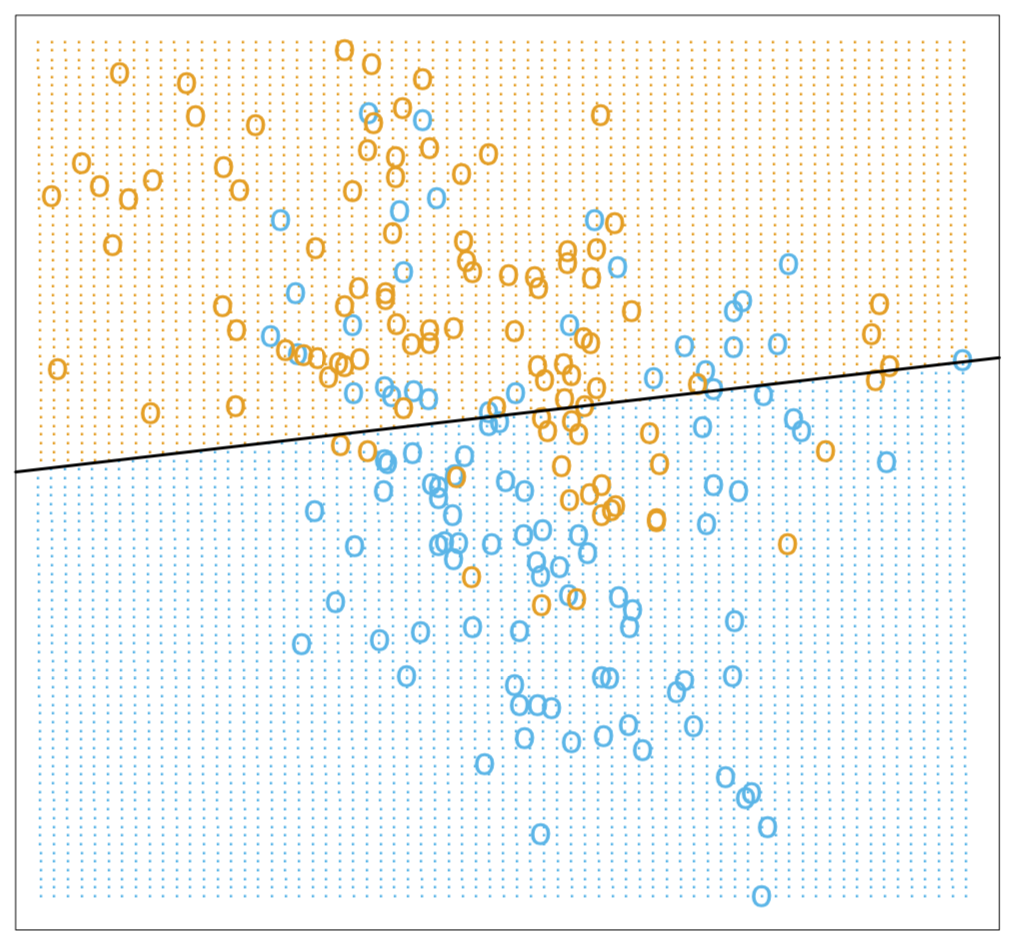
\includegraphics[width=.50\textwidth]{binary_decision_boundary.png} 
    \caption{Example of decision boundary for a binary classifier, from \cite{hastie2009elements}}
    \label{fig:binaryclassifier}
\end{figure}

The Email Spam detection problem described in the last section is a binary classification problem, since the output is binary, either is spam, or isn't. In this work, the focus will be on \textbf{binary classification} problems and its specific metrics.

%% ------------------------------------------------------------------------- %%
\section{Classification Metrics}\index{tree}\index{classifier}\index{metrics}\index{AUC}
\label{classification-metrics}

There are many metrics for model performance and evaluation of classification models. In this study, the metrics evaluated are: the \textit{AUC} (or AUROC), which stands for Area Under the Receiver Operating Characteristic Curve; The logarithmic loss or \textit{Logloss}, which is a commonly used loss function for classification problems; \textit{Brier score}, a score function which measures the accuracy of probabilistic predictions.

In a binary classifier, each prediction of the model is a number between 0 and 1, in the case of LightGBM's binary classification model. For simplicity, assuming that the binary labels are $0$ and $1$, the $\ypred\in [0, 1]$ can be interpreted as the predicted probability of a given instance being of class $1$. In applications where the expected usage is the class itself instead of a probability, a \textbf{threshold} needs to be set, i.e by setting a threshold $\tau$, the predicted labels will be equal to $1$ if $\ypred \geq \tau$, and $0$ otherwise.

The intuition behind choosing these specific metrics are:

\begin{itemize}
    \item AUC is widely used in research, and it's a good metric insensitive to \textit{class imbalance}, having a bounded value between 0 and 1;
    \item Logloss is the direct function optimized in the experiments, i.e. the gradient boosting steps are trying to reduce the logarithmic loss in each step. The logloss takes into account the uncertainty of the prediction and how much the actual label differ from it;
    \item Brier score has good statistical properties, according to \cite{rufibach2010use} it also addresses simultaneously probability calibration, consistency between predicted probabilities and the observation as well as \textit{sharpness}, which is related to the concentration of the predictive distribution;
\end{itemize}

Below an overview about each metric is given, for more information on specific characteristics and mathematical formulation of each evaluation metric one can refer to \cite{BROWN200624}, \cite{rufibach2010use}, \cite{kuhn2013applied} and \cite{hastie2009elements}.

\subsection{AUC}

The Receiver Operating Characteristic curve is probability curve which measures the power of prediction of a binary classifier given a threshold. This curve is done by plotting the \textit{True Positive Rate} (TPR) against the \textit{False Positive Rate}, as seen in Figure \ref{fig:auroc}. They're defined as

$$Roc_x(\tau) = TPR_{\tau} = \frac{TP_{\tau}}{TP_{\tau} + FN_{\tau}}$$
$$Roc_y(\tau) = FPR_{\tau} = \frac{FP_{\tau}}{FP_{\tau} + TN_{\tau}}$$

where TP, FP, TN and FN stands for \textit{True Positives}, \textit{False Positives}, \textit{True Negatives} and \textit{False Negatives}, respectively. All of these metrics depend on the threshold $\tau$. The \textbf{AUC} is defined as the area under this curve, and provides an aggregate measure of the classifier performance against all possible thresholds. It ranges from $0$ (worst performance) to $1$ (perfect classifier).

\begin{figure}[!h]
    \centering
    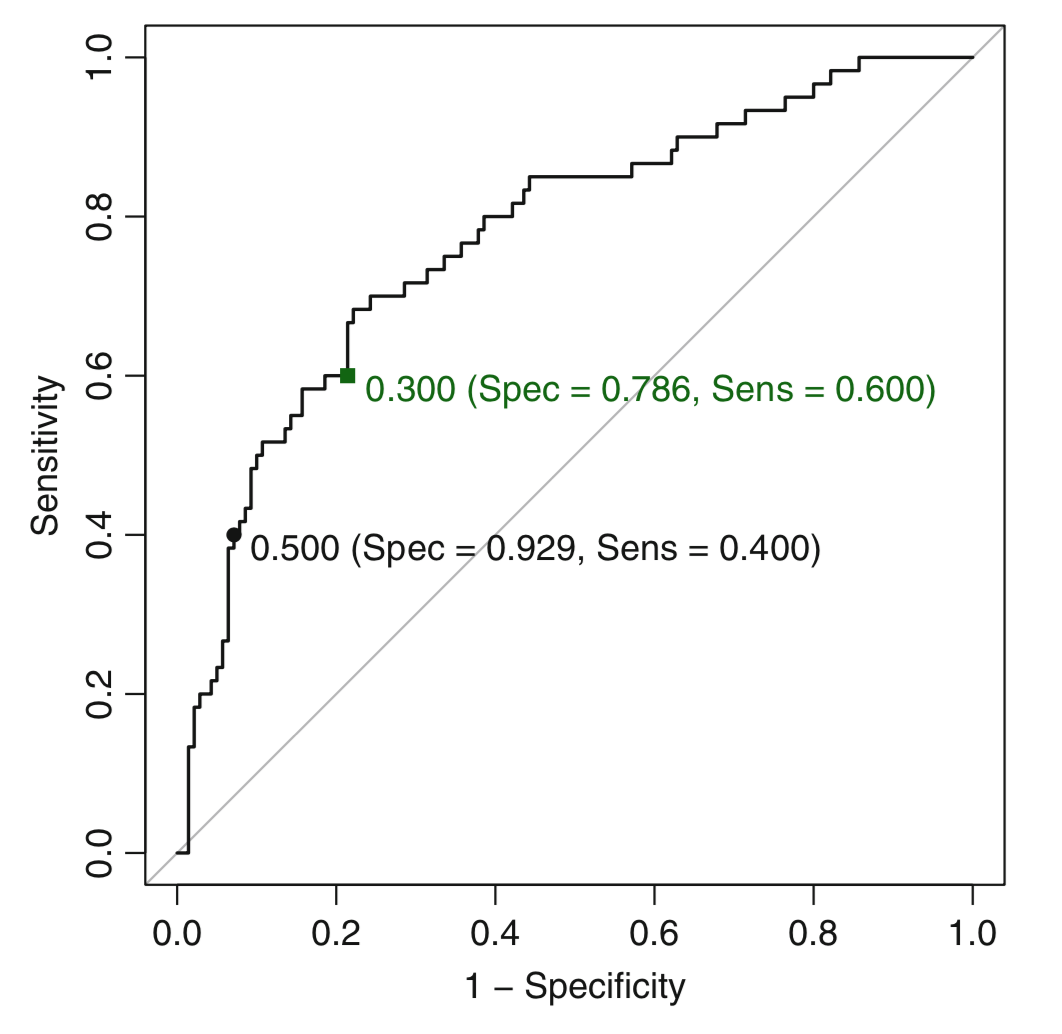
\includegraphics[width=.50\textwidth]{roc_curve.png} 
    \caption{ROC curve of a logistic regression classifier, from \cite{kuhn2013applied}}
    \label{fig:auroc}
\end{figure}

\subsection{Brier Score}

The \textbf{brier score} is the mean squared difference between the predicted probabilities and the actual labels. Similar to the AUC, brier score is a bounded measure from 0 to 1, but it's interpretation and ordering is different: 0 is the best possible brier score, while 1 is the worst. The actual equation is shown in \ref{eq:brier-score}.

Brier score can sum up different components related to forecasting, especially taking into account the calibration of the predicted probabilities. In \cite{murphy1973new} there's an insightful partition of the Brier Score in three components, according to the article: ``a measure of the uncertainty inherent in the events, or states, on the occasions of concern (...); a measure of the reliability of the forecasts; and  a new measure of the resolution of the forecasts''.

\begin{equation}\label{eq:brier-score}
    Brier=\frac{1}{n}\sum_{i=1}^{n}(\yisupred - \yisup)^2
\end{equation}

\subsection{Logloss}

Logarithmic Loss or \textbf{Logloss} measures the accuracy of a classifier by penalizing mistakes depending on how uncertain a prediction is from the actual label. Basically, this encapsulates the intuition that giving a highly confident prediction (e.g. $\ypred = 0.95$) but being very far from the actual label $\ytarget = 0$ is worse then being uncertain about it (e.g.  $\ypred = 0.5$). The logloss equation for binary classifiers is shown in \ref{eq:logloss}

\begin{equation}\label{eq:logloss}
    Logloss = -\frac{1}{N}\sum_{i=1}^{n}[\yisup \log \yisupred + (1 - \yisup)\log(1 - \yisupred)]
\end{equation}




%% ------------------------------------------------------------------------- %%
\section{Model Tuning}\index{tuning}\index{hyperparameter}\index{machine!learning}

Many models in supervised learning have parameters that cannot be directly from the available data. For example, in a decision tree algorithm the max depth or the criterion to measure the quality of a split needs to be chosen before the algorithm learning process. According to \cite{kuhn2013applied} this type of parameter is called a \textit{tuning parameter} because there's no analytical formula available to calculate an appropriate value. This parameter is also called a \textbf{hyperparameter}. 

Usually hyperparameters control the complexity of a model, controlling bias and variance of an algorithm. In the decision tree example, increasing the max depth the learning algorithm can use will increase the complexity of the model, as the tree can learn more complex patterns in data. In the logistic regression model, the regularization parameter (usually denoted $\lambda$) is a hyperparameter of the model, and also controls the complexity of the model. For a more complete explanation of regularization and its importance in predictive modeling refer to Chapter 5 of \cite{hastie2009elements}.

Since the hyperparameters are not directly estimated from the training data, there are different methods to optimize and find the appropriate hyperparameters for a given model. In applied machine learning and data science, a common procedure for model tuning (i.e. finding hyperparameters) usually consists of multiple runs of the same algorithm, but changing the hyperparameter(s) in each run, and evaluating the classifier (or other type of model) in a \textbf{validation set}. This set is different than the \textit{test set} presented in section \ref{sec:validation-evaluation}, as the test set is need to assess the generalization error of the final model after model tuning. 

Besides the traditional separation into train, validation and test set, resampling techniques are also widely used for estimating model performance. The two main flavors of resampling according to \cite{kuhn2013applied} is the \textit{k-Fold Cross-Validation}, where the samples are randomly partitioned into $k$ sets of approximate equal size, and in each iteration $k - 1$ of these folds are used for training and the remaining fold is used for model evaluation (see Figure \ref{fig:cvschema}); And another resampling method is a \textit{bootstrap}, a random sample of the data taken \textit{with replacement}, training a model on the selected samples and evaluating to predict the out-of-bag samples.

\begin{figure}[!h]
    \centering
    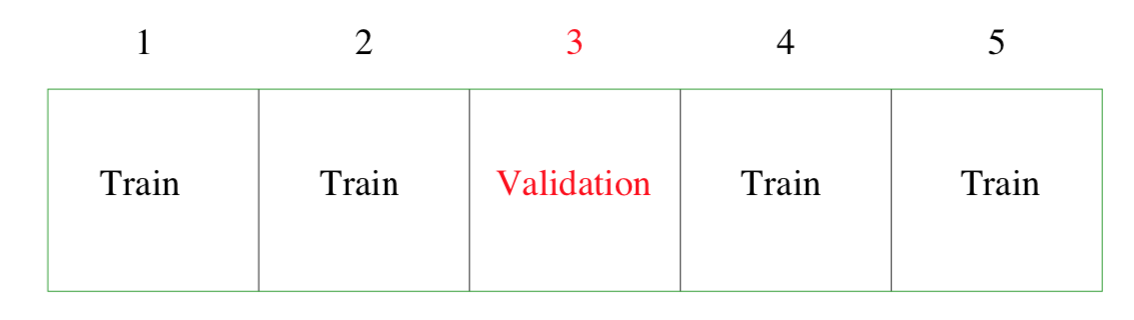
\includegraphics[width=.6\textwidth]{cv_schema.png} 
    \caption{Schema of a single 5-fold Cross-Validation iteration, from \cite{hastie2009elements}}
    \label{fig:cvschema}
\end{figure}

Model tuning is critical part of the workflow when building machine learning models, and there's vast literature exploring different approaches to quantify more sensitive hyperparameters given an algorithm (in \cite{probst2018tunability}), automatic tuning approaches using Bayesian Optimization (\cite{bergstra2013hyperopt}), etc. In this study, the focus is on the hyperparameters of gradient boosting algorithms, specifically gradient boosting with decision trees, explained on Chapter \ref{cap:boosting-intro}.

%% ------------------------------------------------------------------------- %%
\section{Decision Trees}\index{tree}\index{classifier}

Most of the current gradient boosting algorithms use decision trees as the base learners. Decision trees, or specifically \textit{classification trees} in the case of classification problems, consists of multiple nested conditional statements in its internal nodes, with the predictions in the leafs.

The actual learning process of a decision tree is called an \textit{induction} of the decision tree. The idea of the algorithm is to choose internal tree splits that best explain the data and is as small as possible, as described in \cite{aima:2010}. Figure \ref{fig:decision-tree-example} contains an example of a classification tree for deciding wether to wait for a table.

\begin{figure}[!h]
    \centering
    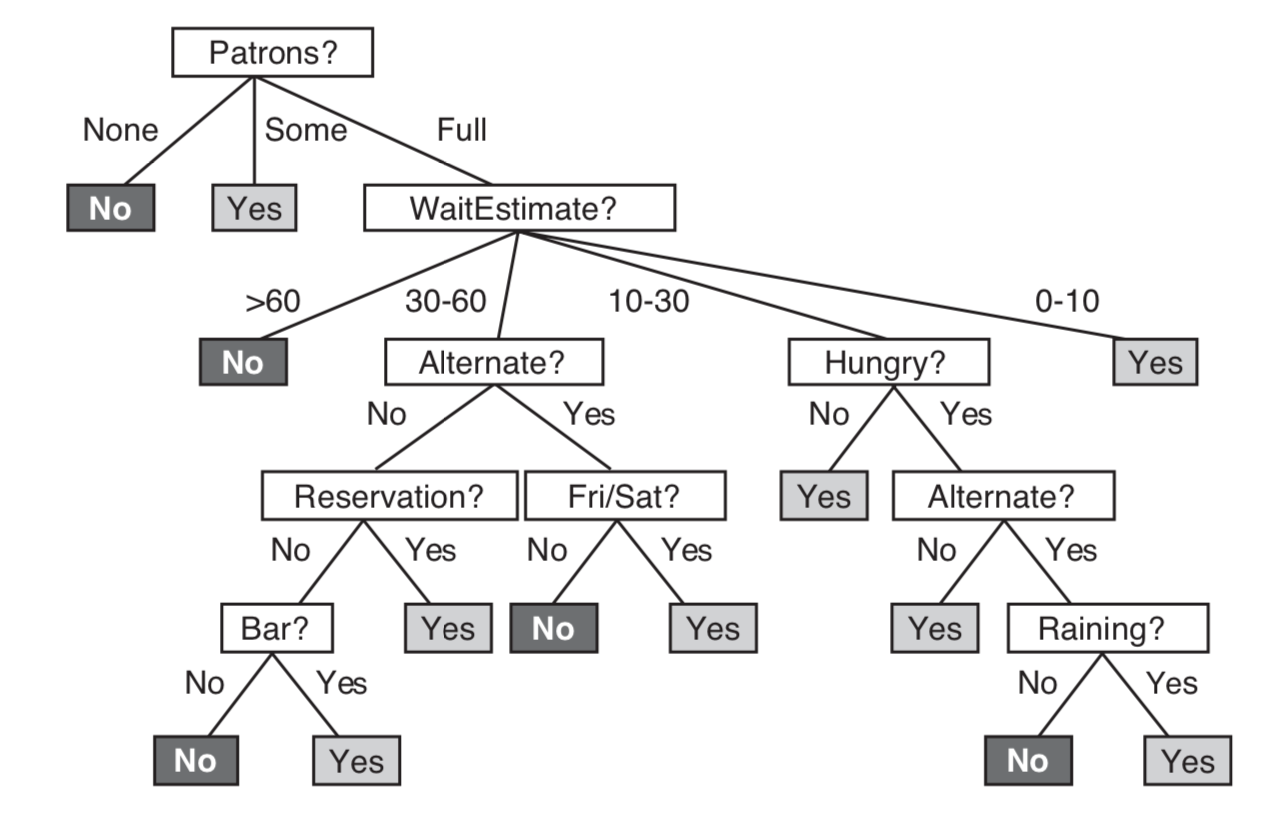
\includegraphics[width=.8\textwidth]{decision-tree-example.png} 
    \caption{Example of a trained decision tree, from \cite{aima:2010}}
    \label{fig:decision-tree-example}
\end{figure}

The learning process of classification trees consists in multiple iterations to choose optimal splits given the training data provided, according to some criteria. Common optimization criteria are usually derived from Information Theory, like the Gini Index, Cross-Entropy and misclassification error. In practical usages and because of numeric properties (see \cite{hastie2009elements}), Gini Index and Cross-Entropy are favored over the misclassification error.

Typical hyperparameters of classifications trees refer to the actual structure of the tree. The \textit{maximum depth} hyperparameter controls how deep the tree can grow, i.e. how many splits will it have, \textit{minimum leaf samples} controls the minimum number of samples each leaf must have, etc. For an extensive empirical study of decision tree hyperparameter tuning, one can refer to \cite{mantovani2018empirical}.
%% ------------------------------------------------------------------------- %%
